\section{Service Composition}
\subsection{Template}
\begin{figure}[h!]
  \centering
  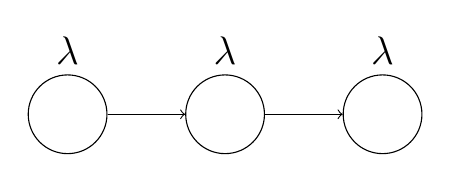
\begin{tikzpicture}
    % Nodes
    \node[draw, circle, minimum size=1cm] (node1) at (0,0) {};
    \node[draw, circle, minimum size=1cm] (node2) at (2,0) {};
    \node[draw, circle, minimum size=1cm] (node3) at (4,0) {};

    % Text on top
    \node[above] at (node1.north) {\Large $\lambda$};
    \node[above] at (node2.north) {\Large $\lambda$};
    \node[above] at (node3.north) {\Large $\lambda$};

    % Connection
    \draw[->] (node1) -- (node2);
    \draw[->] (node2) -- (node3);
  \end{tikzpicture}
  \caption{Service composition template}
  \label{fig:service_composition_template}
\end{figure}

\subsection{Instance}
\begin{figure}[H]
  \centering
  \begin{tikzpicture}
    % Nodes
    \node[draw, circle, minimum size=1cm] (node1) at (0,0) {S1};
    \node[draw, circle, minimum size=1cm] (node2) at (2,0) {S2};
    \node[draw, circle, minimum size=1cm] (node3) at (4,0) {X};
    \node[draw, circle, minimum size=1cm] (node4) at (6,-2) {S3};
    \node[draw, circle, minimum size=1cm] (node5) at (6,2) {S4};
    % Connection
    \draw[->] (node1) -- (node2);
    \draw[->] (node2) -- (node3);
    \draw[->] (node3) -- (node4);
    \draw[->] (node3) -- (node5);
  \end{tikzpicture}
  \caption{Service composition instance}
  \label{fig:service_composition_instance}
\end{figure}
\[ \forall S \in \mathrm{S}_{C}  \exists  \lambda(S) = \mathrm{S}_{1} \]